\newgeometry{top=1cm, bottom=2cm}
\section{Matrizen}
\begin{figure}[h!]
    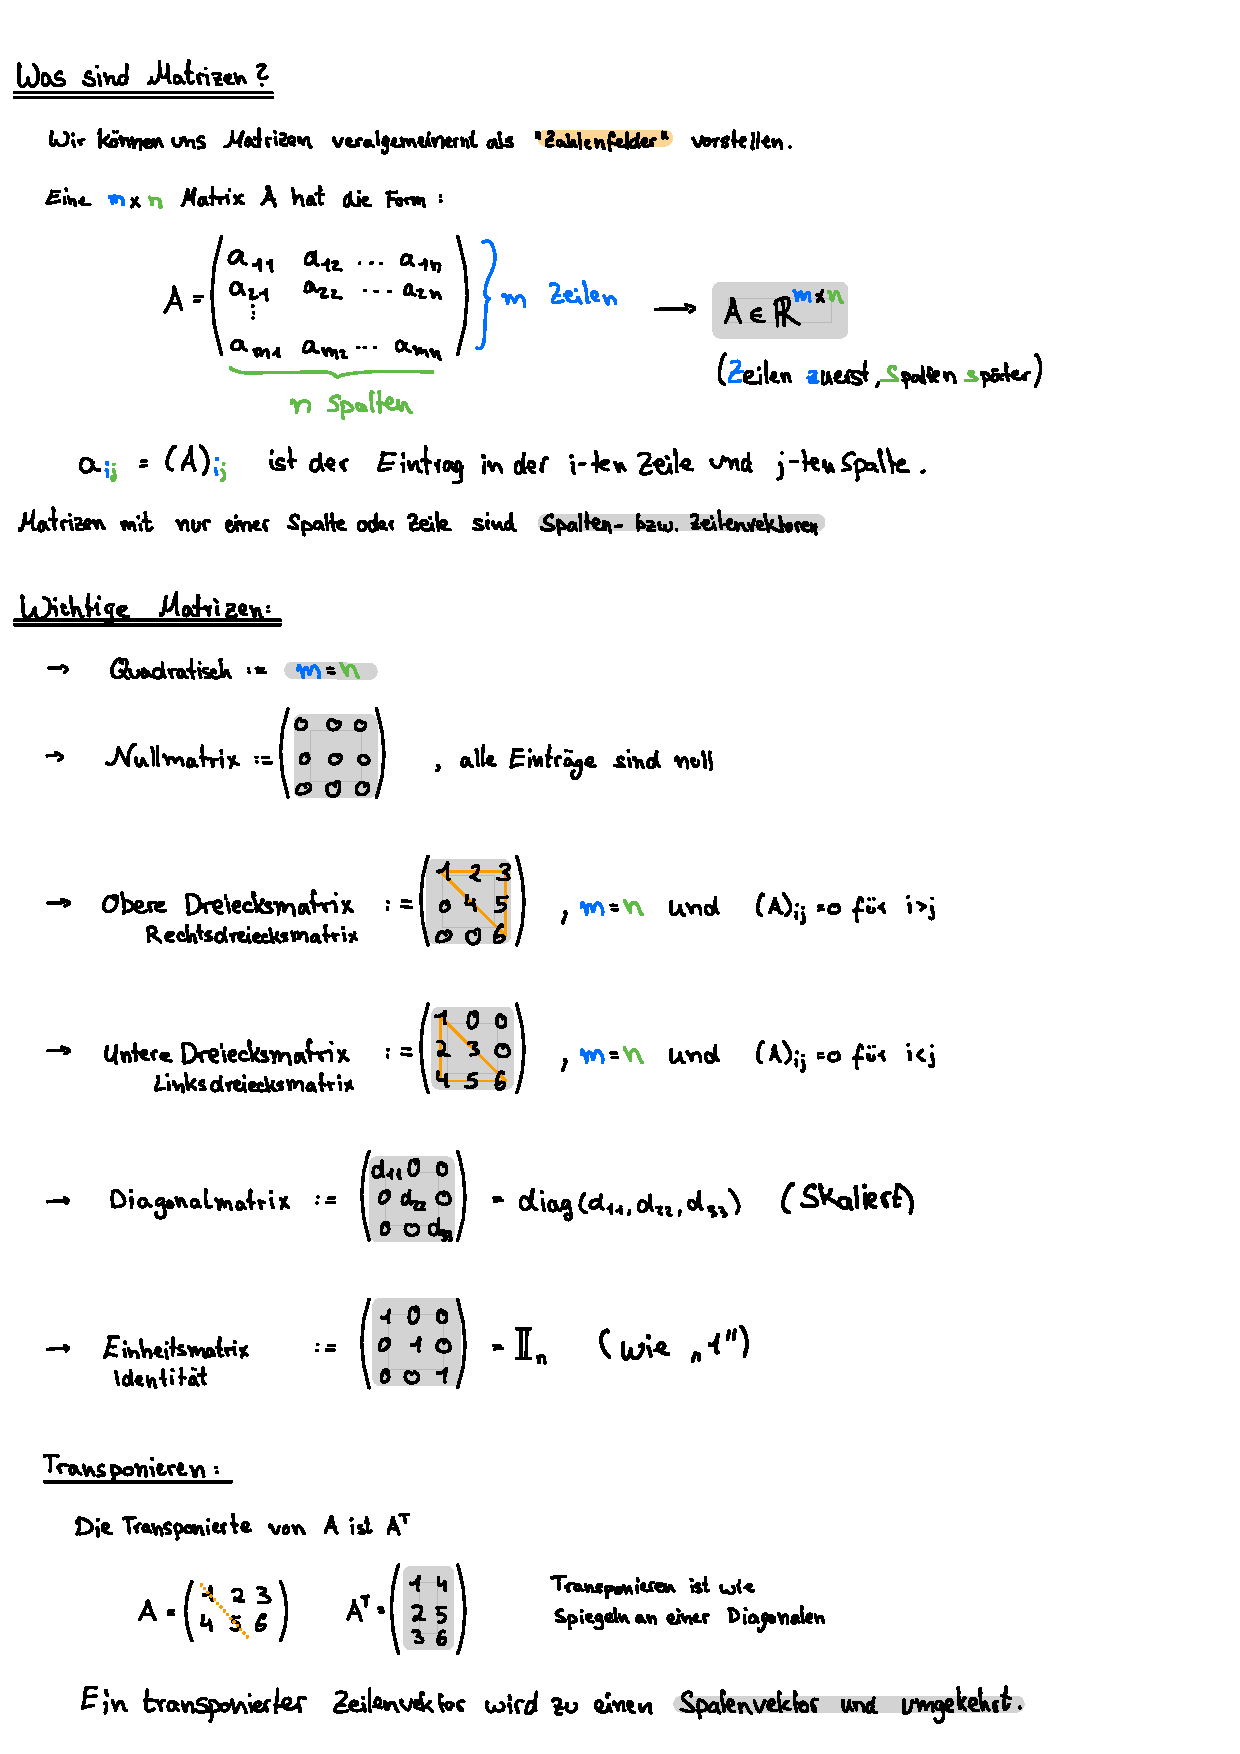
\includegraphics[page=1, scale=0.842]{pdf/02_Matrizen.pdf}
\end{figure}
\newpage
\includepdf[pages={2-}, 
            pagecommand={\thispagestyle{plain}}, 
            scale=0.95]{pdf/02_Matrizen.pdf}

\newgeometry{top=2.5cm, bottom=2cm}
\subsection{Beispielaufgaben} %Übung 06
\vspace{1cm}
\subsubsection{}
Was ist
\[
\begin{pmatrix}
0 & 0 & 1 & 0
\end{pmatrix}
\begin{pmatrix}
-1 & 1 & -1 & 2 \\
0 & 2 & 0 & -1 \\
-3 & 2 & -3 & 1 \\
2 & 1 & 2 & 3 \\
\end{pmatrix}
\begin{pmatrix}
-1 & 1 & -1 & 2 \\
0 & 2 & 0 & -1 \\
-3 & 2 & -3 & 1 \\
2 & 1 & 2 & 3 \\
\end{pmatrix}
\begin{pmatrix}
0\\
1\\
0\\
0\\
\end{pmatrix}?
\]

\textbf{Lösung:}

\newpage
\subsubsection{} %Adi PVK Tag 1
Für $a \in \mathbb{R}$  sei die Matrix
\[
A = \begin{pmatrix}
1 & 0 & 0 & 2 \\
0 & 1 & 0 & 0 \\
-1 & 0 & 1 & 0 \\
a & 1 & 0 & 1 \\
\end{pmatrix}
\]
gegeben. Für welche Werte von $a$ ist die Matrix $A$ singulär bzw. regulär? Bestimmen Sie für $a = 0$ die Inverse von $A$. \\

\noindent \textbf{Lösung:}

\newpage
\subsubsection{} %Zardini S.27
Bestimmen Sie die LR-Zerlegung der Matrix $A$, so dass $LR = PA$
\[
A = \begin{pmatrix}
0 & 1 & -3 \\
-3 & 7 & 6 \\
-3 & -2 & -2 \\
\end{pmatrix}.
\]

\textbf{Lösung:}